\documentclass[UTF8]{ctexart}
\usepackage[paperwidth=9cm,paperheight=22cm,margin=6mm]{geometry}
\usepackage{graphicx}
\pagestyle{empty}
\begin{document}
\begin{center}
\vbox{\centering
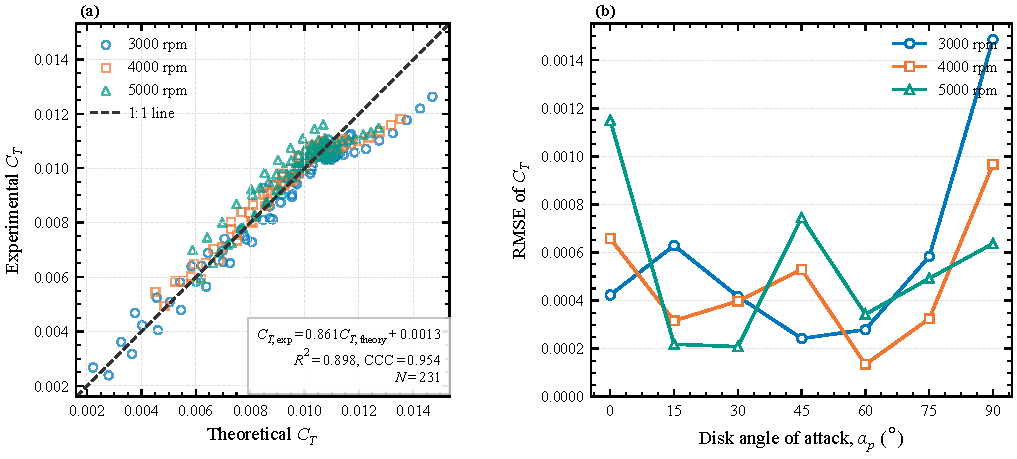
\includegraphics[width=7.5cm]{Image/fig9_rotor_model_diagnostics.pdf}\\[1mm]
{\small 图7\quad 升力系数一致性与攻角分区相对误差分布
\\ Fig.\,7 \quad Thrust coefficient agreement and relative-error distributions by disk angle of attack}\\[1mm]
\parbox{0.98\columnwidth}{\scriptsize 注：共231个工况，197/231的绝对相对误差不超过10\%。(a)参考线为1:1及相对实测值的$\pm10\%$误差边界。(b)相对误差为实测$C_T$减理论$C_T$，再除以实测$C_T$，正值表示模型低估，负值表示模型高估。每个攻角包含33个工况，全部数据均参与箱线图计算；箱体为第25--75百分位区间，箱内横线为中位数，须线延伸至1.5倍四分位距范围内的最远数据点，未显示须线外离群点标记。箱线图反映工况间分布，不表示重复试验的置信区间。}
}
\end{center}

\end{document}
